\section{Quantitative Evaluation} 

In this section we describe an experiment we ran to evaluate whether VeriCAT improves users' ability to identify when Russian $\rightarrow$ English translated text is of sufficiently low quality to be untrustworthy. The following sections outline the study in more detail. 

%\subsection{Explanation Techniques}
\subsection{Experimental Conditions}

We perform a between-subjects 3 condition experiment. In the baseline condition, participants see a passage of original Russian text broken into sentences, along with the corresponding MT. No additional information is provided to the participant. Essentially, the baseline condition is the VeriCAT interface without quality scores. We chose this as our baseline (as opposed to raw input and output to the FairSeq translation model) to avoid confounding the benefits of VeriCAT with the benefits of clean text formatting. % keep the baseline condition as consistent with other conditions as possible.    

In addition to the baseline condition, we include two experimental conditions, each of which incorporates a version of VeriCAT. 
In the first experimental condition, participants use the VeriCAT system with quality scores output by its QE model (Figure \ref{fig:p3_predicted_quality}) to perform the experimental task. 
In the second experimental condition, participants use the VeriCAT interface, but instead of showing predicted quality scores, the interface shows human-generated direct assessment (DA) scores of the translated text (Figure \ref{fig:p1_human_quality}). 
We refer to the experimental conditions as Predicted Quality (for VeriCAT with its QE model scores), and Human Quality (for the VeriCAT interface, with DA scores). 

In the event that VeriCAT fails to improve participants' performance, we want to design the experiment such that we can distinguish between failure due to the system design vs. failure due to variance in predicted quality scores. In other words, we include the Human Quality condition so that we can rule out variance in predicted quality scores as a mode of failure. 

\subsection{Passage Type}
We postulate that without quality scores, users will rely on fluency as a proxy for translation quality. Prior work shows that this is the case when it comes to trust of MT \cite{martindaleFluency2018}. However, there are cases where this technique fails, as described in Section \ref{sec:design_requirements}.  
In our experiment, each translated sentence falls into one of four categories: (1) \textit{poor fluency + poor quality}, (2) \textit{poor fluency + good quality}, (3) \textit{good fluency + poor quality}, (4) \textit{good fluency + good quality}. We expect sentences in the \textit{good fluency + poor quality}, and \textit{poor fluency + good quality} categories to be the most difficult for participants to assess. To balance the experiment with these different sentence types we arrange two different types of passages described below: 

\begin{compacthang}
    \item \textbf{Type 1} \textit{Good fluency + good quality, good fluency + poor quality, poor fluency + good quality}. Passage 1 is of this type and is shown in Figure \ref{fig:p1_human_quality}.    
    \item \textbf{Type 2} \textit{Good fluency + good quality, poor fluency + good quality, poor fluency + poor quality}. Passage 3 is of this type and is shown in Figure \ref{fig:p3_predicted_quality}.     
\end{compacthang}

Both of these passage types are designed to test if participants will heed quality scores or (their own intuition based on) fluency, as a primary indicator of poor quality translation. 

\subsection{Task} 
We run a 3 condition experiment: Baseline, Human Quality, and Predicted Quality. Within each condition we include 2 passages of type 1 followed by 2 of type 2. The experimental task replicates a user determining if a MT needs a human translation as closely as possible within a controlled setting. 

\begin{table}[h!]
\resizebox{0.50\textwidth}{!}{%
\begin{tabular}{c|c|c}
\hline
\begin{tabular}[c]{@{}c@{}}Human Quality Score \\ (Human Quality)\end{tabular} & \begin{tabular}[c]{@{}c@{}}Predicted Quality Score \\ (Predicted Quality)\end{tabular} &  \begin{tabular}[c]{@{}c@{}}Baseline\\ (Baseline)\end{tabular} \\ \hline
                                                                    59                                                                       & 59                                                                                         & 47                                                        \\ \hline
\end{tabular}
}
\caption{N for each condition. }
\label{tab:exp_N}
\end{table}

Participants are shown four passages of text. Within each passage, text is broken into three sentences. For each sentence, we show the original Russian text and the FairSeq English translation. Participants in either of the quality score conditions also see a quality score for each sentence (Figure \ref{fig:exp_stim}). Participants are instructed to decide if any of the sentences in the passage should be re-translated by a human and are given the chance to select sentence 1, 2, or 3 of the passage for re-translation by a human, or to opt for no-retranslation. After this selection, the original passage and machine translation remain on the screen and the human translation of whichever sentence they selected is shown. At this point, participants are asked to answer two information retrieval questions. 
 %The prompt before each passage is as follows:

%\begin{quote}
%Below is a passage written in Russian with an English translation generated by artificial intelligence. When you are ready, you will be asked to answer two comprehension questions. \textbf{You may select up to one section of the passage for re-translation by a human.} We recommend selecting the section you judge to have the poorest machine translation for re-translation by a human. 

%Click ``I’m ready to see the questions'' when you are ready to see the comprehension questions. \textbf{If you would like a human re-translation of any section of the passage you must request it BEFORE you click ``I’m ready to see the questions''.} Once you click ``I’m ready to see the questions'', comprehension questions will appear on the page alongside the Russian test, English Machine translation, and any human translations you requested.  
%\end{quote}


\subsection{Participants} 

We recruited 193 participants from Amazon Mechanical Turk. Participation was restricted to workers in the United States with an approval rating of greater than 90 percent who do not speak Russian or Ukrainian. Participants were paid a base rate of USD $1.60$ for participation. Before analysis, participants who answered information retrieval questions for passage 1 and passage 2 (attention check questions) incorrectly were dropped from analysis ($N = 28$).  This left $N = 165$ participants distributed among stimuli as shown in Table \ref{tab:exp_N}. Demographics of participants are shown in Table \ref{tab:exp_demo}.


\begin{table}[h!]
\begin{threeparttable}[b]
\begin{tabular}{ll}
\hline
N                                                                                & 165                                                                                                                                                    \\ \hline
Age                                                                              & \begin{tabular}[c]{@{}l@{}}18-24: 6.7\%, 25-34: 45.5\%, 35-44: 24.8\%, \\ 45-54: 14.5\%, 55-64: 7.3\%, 65+: 1.2\%\end{tabular}                                     \\ \hline
Gender                                                                           & \begin{tabular}[c]{@{}l@{}}Female: 38.2\%, Male: 61.2\%, Non-binary: 0.6\%\end{tabular}                                                             \\ \hline
Education                                                                        & \begin{tabular}[c]{@{}l@{}}High School: 13.3\%, Associates: 12.1\%, Bachelors: 60.0\%, \\ Masters: 11.5\%, Professional: 2.4\%, Doctorate: 0.6\%\end{tabular}                            \\ \hline
\end{tabular}
\end{threeparttable}
\caption{Participant demographics.}
\label{tab:exp_demo}
\end{table}

\subsection{Procedure}

The experiment follows an approved protocol per \textit{redacted for anonymity}’s company policy and was posted as a HIT on Amazon Mechanical Turk. Workers who accept the HIT follow a link to the experiment. After providing informed consent, participants see an instruction page explaining the experiment. This page explains that they will see 4 passages of text translated from Russian to English by AI and that they will be asked to answer two comprehension questions for each passage. The instructions also explain that before seeing the comprehension questions the participant will have the opportunity to select one of the sentences in the passage for re-translation by a human. After the instruction page, participants see the four passages one at a time. They can take as much time as they need before clicking a button to select which section of the passage they want to re-translate and viewing the passage questions. After completing the main task, participants complete a short post-experiment questionnaire, the Tolerance for Ambiguity Survey from Geller et al. 1993 \cite{gellerTolerance1993}, a short demographic questionnaire, and have the option to provide any additional feedback.

\subsection{Hypotheses}

%We postulate that providing quality estimations for each sentence will help participants identify the sentence of lowest quality for re-translation only in cases where there is a significant difference between scores. In other words, we expect participants in the Human Quality condition to perform significantly better than participants in the Predicted Quality condition. 

%We evaluate VeriCAT with DA vs. QE scores, and with respect t our design requirements (Section \ref{sec:design_requirements}). To gather a more nuanced understanding of how individual users may or may not benefit from our approach to explaining MT we also test a number of hypotheses based on individual user differences. 

We analyse the results of this experiment according to the following hypotheses: 


\begin{compacthang}
    \item \textbf{H1}: Participants in the VeriCAT (with quality scores) conditions will have higher accuracy in identifying which sentence in a passage is of low quality and should be re-translated than participants in the baseline condition. 
    \item \textbf{H2}: Participants in the VeriCAT (with quality scores) conditions will have a greater change in trust of machine translation than participants in the baseline condition. 
    \item \textbf{H3}: Participants’ tolerance for ambiguity will correlate with how well they are able to use VeriCAT (with quality scores) to perform the experimental task.
    \item \textbf{H4}: Participants’ experience using machine translation will correlate with how well they are able to use VeriCAT (with quality scores) to perform the experimental task.
    \item \textbf{H5}: Participants’ self-rated expertise in AI, MT, visualization, and statistics will correlate with how well they are able to use VeriCAT (with quality scores) to perform the experimental task.   
\end{compacthang}

\begin{figure}*
    \centering
    
    \cbox{bar-noXai} \textit{Baseline} \quad
    \cbox{bar-Qual} \textit{Human Quality} \quad
    \cbox{bar-PredictQ} \textit{Predicted Quality} \quad
    
    \begin{subfigure}[t]{0.45\textwidth}
        \centering
        \scalebox{0.7}{
        \begin{bchart}[step=.25,max=1,width=\linewidth]
        \bcbar[color=bar-noXai]{.06}
        \bclabel{\textit{Good Fluency}}
        \bcbar[color=bar-Qual]{.51}
        \bclabel{\textit{Poor score}}
        \bcbar[color=bar-PredictQ]{.37}
        \bcskip{6pt}
        
        \bcbar[color=bar-noXai]{.15}
        \bclabel{\textit{Good Fluency}}
        \bcbar[color=bar-Qual]{.15}
        \bclabel{\textit{Good score}}
        \bcbar[color=bar-PredictQ]{.07}
        \bcskip{6pt}
        
        \bcbar[color=bar-noXai]{.38}
        \bclabel{\textit{Poor Fluency}}
        \bcbar[color=bar-Qual]{.14}
        \bclabel{\textit{Good score}}
        \bcbar[color=bar-PredictQ]{.31}
        \bcskip{6pt}
        
        \bcbar[color=bar-noXai]{.40}
        \bclabel{\textit{No}}
        \bcbar[color=bar-Qual]{.20}
        \bclabel{\textit{Re-translation}}
        \bcbar[color=bar-PredictQ]{.25}
        
        \bcxlabel{Proportion of Participants Selecting}
        \end{bchart}}
        \caption{Passage 1} 
        \label{fig:exp_p1_prop_answers}
    \end{subfigure}
    \hfill
    \begin{subfigure}[t]{0.45\textwidth}
        \centering
        \scalebox{0.7}{
        \begin{bchart}[step=.25,max=1,width=\linewidth]
        \bcbar[color=bar-noXai]{.06}
        \bclabel{\textit{Good Fluency}}
        \bcbar[color=bar-Qual]{.53}
        \bclabel{\textit{Poor score}}
        \bcbar[color=bar-PredictQ]{.37}
        \bcskip{6pt}
        
        \bcbar[color=bar-noXai]{.13}
        \bclabel{\textit{Good Fluency}}
        \bcbar[color=bar-Qual]{.12}
        \bclabel{\textit{Good score}}
        \bcbar[color=bar-PredictQ]{.08}
        \bcskip{6pt}
        
        \bcbar[color=bar-noXai]{.21}
        \bclabel{\textit{Poor Fluency}}
        \bcbar[color=bar-Qual]{.15}
        \bclabel{\textit{Good score}}
        \bcbar[color=bar-PredictQ]{.20}
        \bcskip{6pt}
        
        \bcbar[color=bar-noXai]{.60}
        \bclabel{\textit{No}}
        \bcbar[color=bar-Qual]{.20}
        \bclabel{\textit{Re-translation}}
        \bcbar[color=bar-PredictQ]{.34}
        
        \bcxlabel{Proportion of Participants Selecting}
        \end{bchart}}
        \caption{Passage 2} 
        \label{fig:exp_p2_prop_answers}
    \end{subfigure}
    \hfill
     \begin{subfigure}[t]{0.45\textwidth}
        \centering
        \scalebox{0.7}{
        \begin{bchart}[step=.25,max=1,width=\linewidth]
        \bcbar[color=bar-noXai]{.26}
        \bclabel{\textit{Poor Fluency}}
        \bcbar[color=bar-Qual]{.69}
        \bclabel{\textit{Poor score}}
        \bcbar[color=bar-PredictQ]{.68}
        \bcskip{6pt}
        
        \bcbar[color=bar-noXai]{.19}
        \bclabel{\textit{Poor Fluency}}
        \bcbar[color=bar-Qual]{.05}
        \bclabel{\textit{Good score}}
        \bcbar[color=bar-PredictQ]{.15}
        \bcskip{6pt}
        
        \bcbar[color=bar-noXai]{.09}
        \bclabel{\textit{Good Fluency}}
        \bcbar[color=bar-Qual]{.10}
        \bclabel{\textit{Good score}}
        \bcbar[color=bar-PredictQ]{.03}
        \bcskip{6pt}
        
        \bcbar[color=bar-noXai]{.47}
        \bclabel{\textit{No}}
        \bcbar[color=bar-Qual]{.15}
        \bclabel{\textit{Re-translation}}
        \bcbar[color=bar-PredictQ]{.14}
        
        \bcxlabel{Proportion of Participants Selecting}
        \end{bchart}}
        \caption{Passage 3} 
        \label{fig:exp_p3_prop_answers}
    \end{subfigure}
    \hfill
    \begin{subfigure}[t]{0.45\textwidth}
        \centering
        \scalebox{0.7}{
        \begin{bchart}[step=.25,max=1,width=\linewidth]
        \bcbar[color=bar-noXai]{.45}
        \bclabel{\textit{Poor Fluency}}
        \bcbar[color=bar-Qual]{.64}
        \bclabel{\textit{Poor score}}
        \bcbar[color=bar-PredictQ]{.64}
        \bcskip{6pt}
        
        \bcbar[color=bar-noXai]{.02}
        \bclabel{\textit{Poor Fluency}}
        \bcbar[color=bar-Qual]{.12}
        \bclabel{\textit{Good score}}
        \bcbar[color=bar-PredictQ]{.08}
        \bcskip{6pt}
        
        \bcbar[color=bar-noXai]{.11}
        \bclabel{\textit{Good Fluency}}
        \bcbar[color=bar-Qual]{.10}
        \bclabel{\textit{Good score}}
        \bcbar[color=bar-PredictQ]{.12}
        \bcskip{6pt}
        
        \bcbar[color=bar-noXai]{.43}
        \bclabel{\textit{No}}
        \bcbar[color=bar-Qual]{.14}
        \bclabel{\textit{Re-translation}}
        \bcbar[color=bar-PredictQ]{.15}
        
        \bcxlabel{Proportion of Participants Selecting}
        \end{bchart}}
        \caption{Passage 4} 
        \label{fig:exp_p4_prop_answers}
    \end{subfigure}
    
    \caption{Proportions of participants selecting each type of sentence for re-translation by passage.}
    \label{fig:exp_prop_answers}

\end{figure}

\subsection{Findings}

We consider participants' answers correct if they select the sentence with the lowest quality score to be re-translated. In all cases, the sentence with the lowest score in the predicted quality score condition is the same as the sentence with the lowest score in the human quality score condition. To calculate overall user performance accuracy, we sum the number of correct answers across all four passages and divide by 4. The following analyses use this outcome measure to test the hypotheses listed above. Analysis scripts and de-identified data are available in supplemental materials. 

\subsubsection{\textbf{Does VeriCAT help?}}

We start by looking at which sentences people chose to re-translate for each condition and passage. For all passages, we see participants in the quality score conditions are, on average, most accurate at selecting the correct sentence for re-translation. Interestingly, we see that participants in the baseline condition often opt for no-retranslation. Proportions of participants giving each answer for each passage and condition are shown in Figure \ref{fig:exp_prop_answers}.

To test if the differences we observe are significant we run a Kruskal-Wallis test of $overall\_score \sim condition$ \footnote{We use a Kruskal-Wallis test because according to the Shapiro-Wilk Normality test $overall\_score$ is not normally distributed ($W = 0.87, p < 0.001$).} and find a significant difference across conditions ($H(2) = 29.7, p < 0.001$). A post-hoc Dunn’s multiple comparisons test with a Bonferroni corrected alpha ($0.02$) shows significant pairwise differences between Human Quality and baseline ($Z = 5.2, p < 0.01$), and baseline and Predicted Quality ($Z = -4.3, p < 0.01$). Figure \ref{fig:exp_overall_distribution} shows $overall\_score$ distributions by condition. 

\begin{figure}[h!]
  \centering
  \begin{minipage}[b]{0.45\textwidth}
    
   %\begin{figure}[h!]
    %\centering
    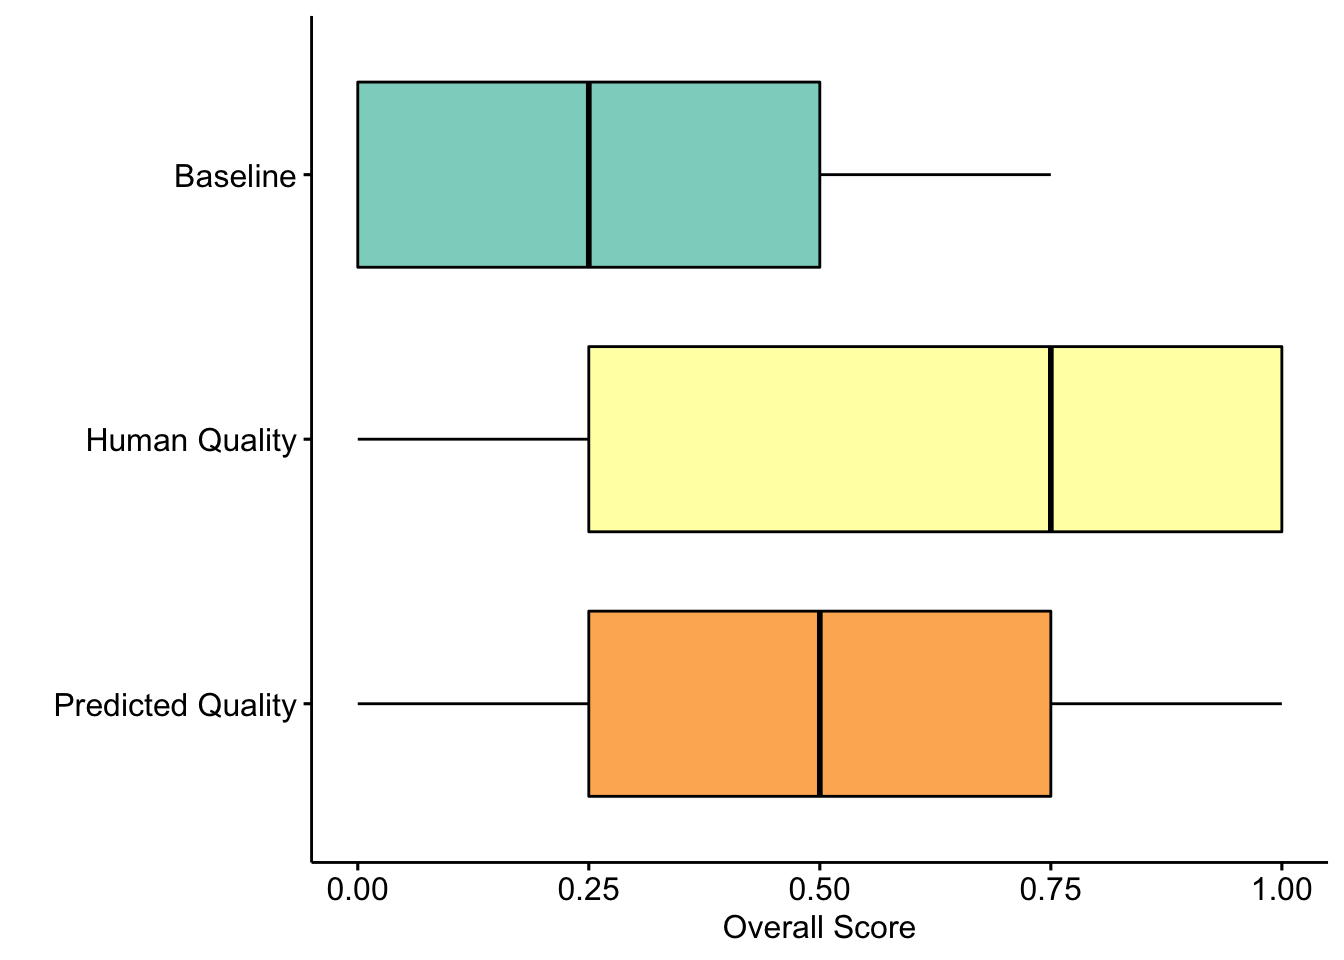
\includegraphics[width=0.95\textwidth]{exp2_overall_distribution.png}
    \caption{Boxplot of overall score by condition.}
    \label{fig:exp_overall_distribution}
    %\end{figure}
    
  \end{minipage}
  \hfill
  \begin{minipage}[b]{0.45\textwidth}
  
    %\begin{figure}[h!]
    %\centering
    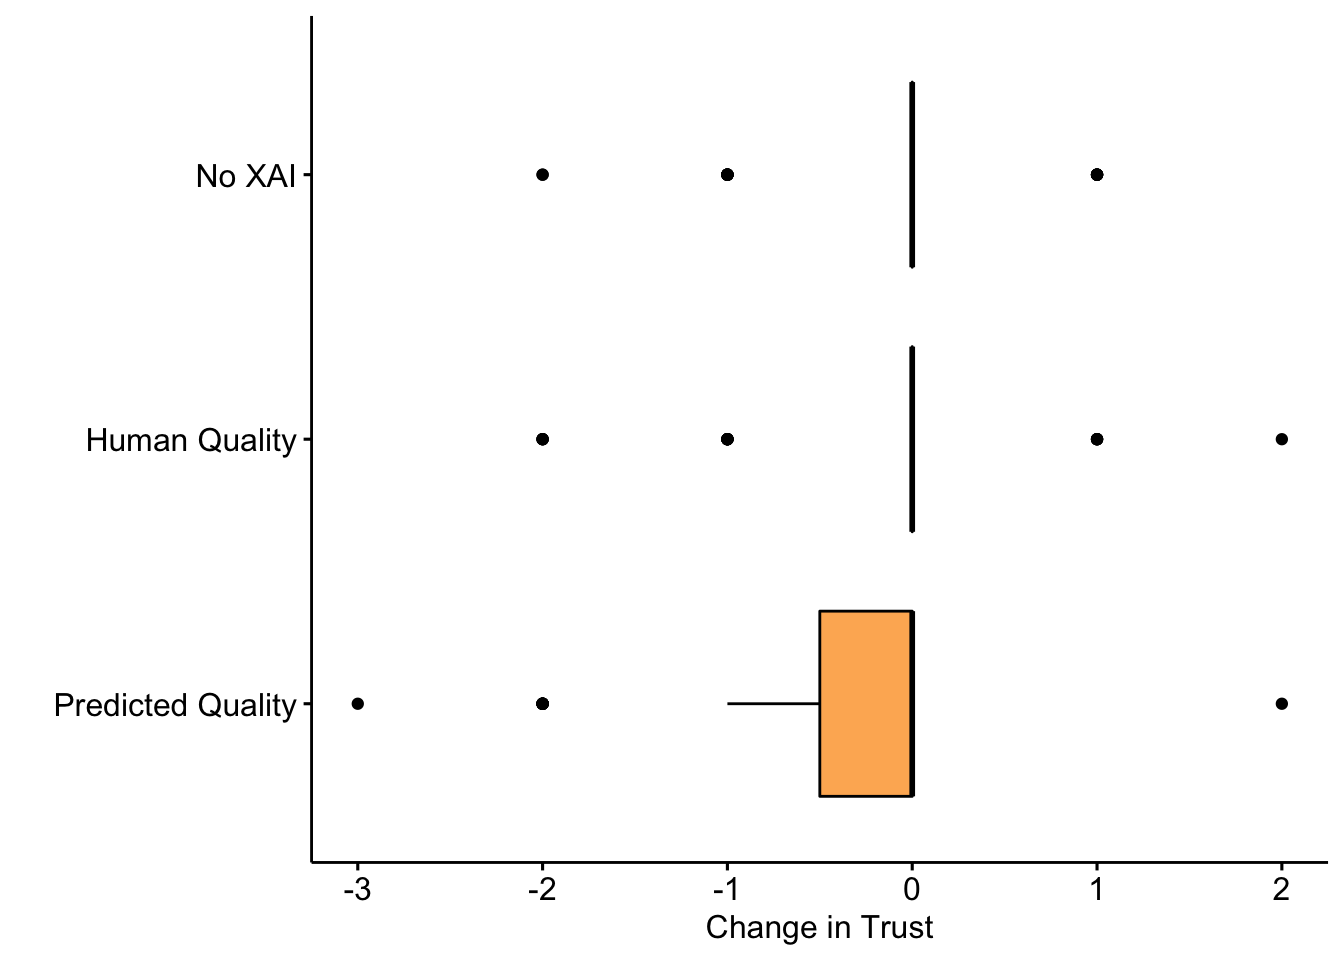
\includegraphics[width=0.95\textwidth]{exp2_delta_trust.png}
    \caption{Boxplot of change in trust by condition.}
    \label{fig:exp_delta_trust}
    %\end{figure}
    
  \end{minipage}
\end{figure}

These results suggest that VeriCAT's sentence-level quality scores can significantly improve participants’ performance over baseline, regardless of whether the scores come from (noisy) predictions generated by the QE model, or human judgments (DA scores). Therefore, we \textbf{accept H1}. The results also do not indicate a significant difference in performance between predicted quality scores and human quality scores. We interpret this to suggest that, though imperfect, VeriCAT's predicted quality scores are comparable to the human quality scores in their impact on users' ability to perform the task. 

\subsubsection{\textbf{Does VeriCAT affect trust?}}

Before the experimental task, we ask participants: “Please rate how much you trust artificial intelligence to correctly translate sentences from a language you do not speak into a language you do speak from 1 (No trust) to 5 (Complete trust).”  We ask the same question again at the end of the experiment. To analyze whether different conditions inspire a change in participants' reported trust, we calculate $delta\_trust$ for each participant by subtracting their answer to the pre-experimental task trust question from their answer to the post-experimental task trust question. 

We run a Kruskal-Wallis test of $delta\_trust \sim condition$ \footnote{We use a Kruskal-Wallis test because according to the Shapiro-Wilk Normality test $delta\_trust$ is not normally distributed ($W = 0.74, p < 0.001$).} and find no significant difference across conditions ($H(2) = 3.5, p = 0.17$). This suggests that neither Human Quality or Predicted Quality scores significantly affect participants’ trust in machine translation, thus we \textbf{reject H2}. Average change in trust by condition is shown in Figure \ref{fig:exp_delta_trust}.

\subsubsection{\textbf{Is the efficacy of VeriCAT influenced by participants' individual differences?}}

Prior work indicates that individual user differences can play a strong role in how well users utilize a visualization for a problem solving task\cite{liuSurvey2020}. However, there is little research investigating how individual differences can affect understanding, trust, and use of AI. In an effort to investigate this question, we capture three different individual differences of participants (intolerance for ambiguity, usage of MT, and self-rated expertise) and analyse whether there are any correlations between these measures and participants’ $overall\_score$. Our findings follow.

\begin{figure}[h!]
  \centering
  
    \cbox{bar-noXai} \textit{Baseline} \quad
    \cbox{bar-Qual} \textit{Human Quality} \quad
    \cbox{bar-PredictQ} \textit{Predicted Quality} \quad
    
  \begin{minipage}[b]{0.45\textwidth}
    
   %\begin{figure}[h!]
    %\centering
    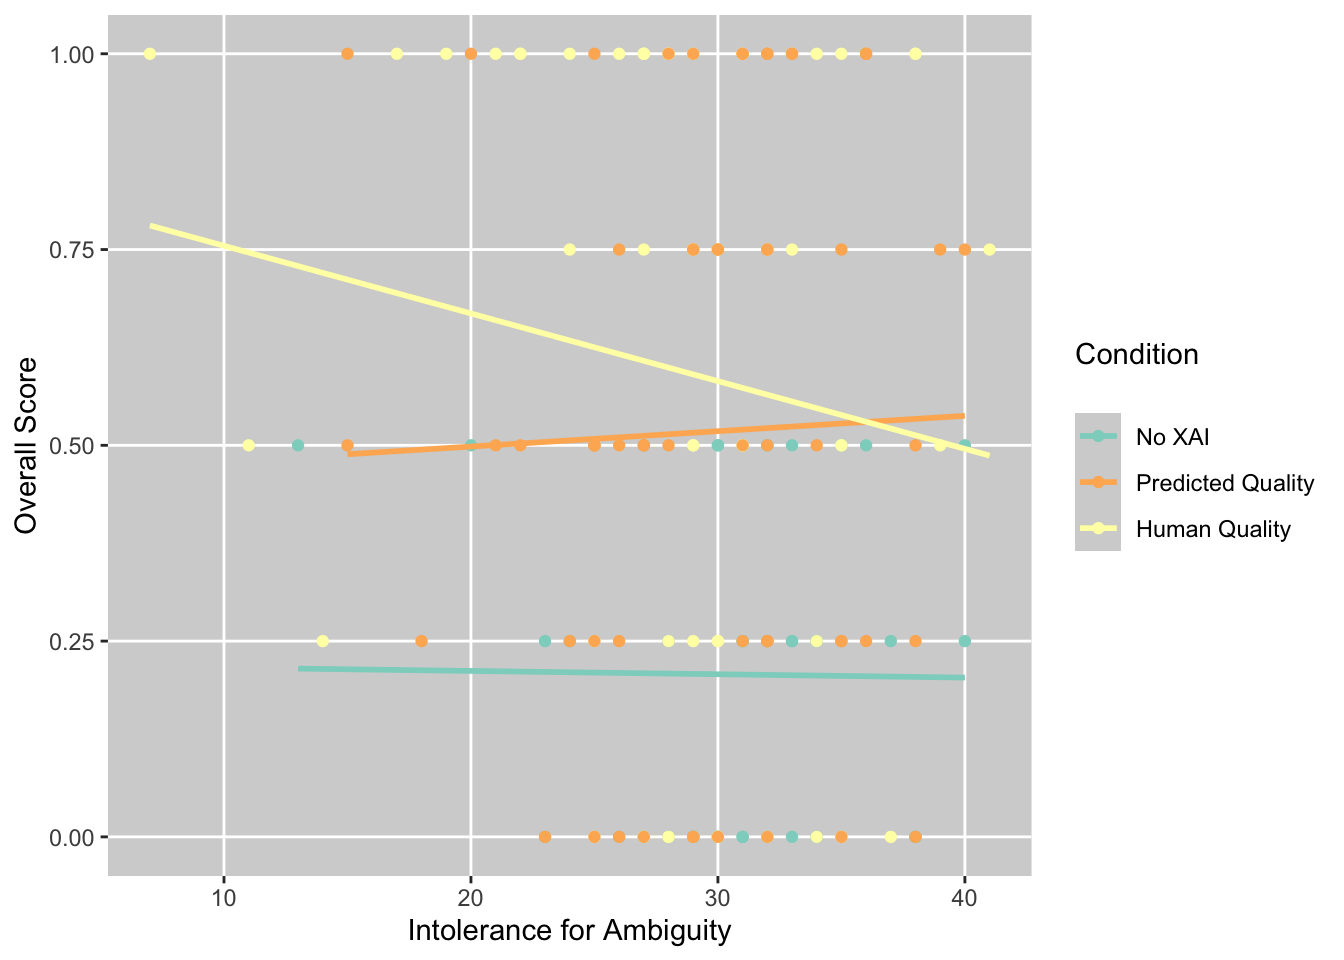
\includegraphics[width=0.95\textwidth]{exp2_intol_ambiguity.png}
    \caption{Regression lines of overall score and intolerance for ambiguity by condition.}
    \label{fig:exp_intol_ambiguity}
    %\end{figure}
    
  \end{minipage}
  \hfill
  \begin{minipage}[b]{0.45\textwidth}
  
    %\begin{figure}[h!]
    %\centering
    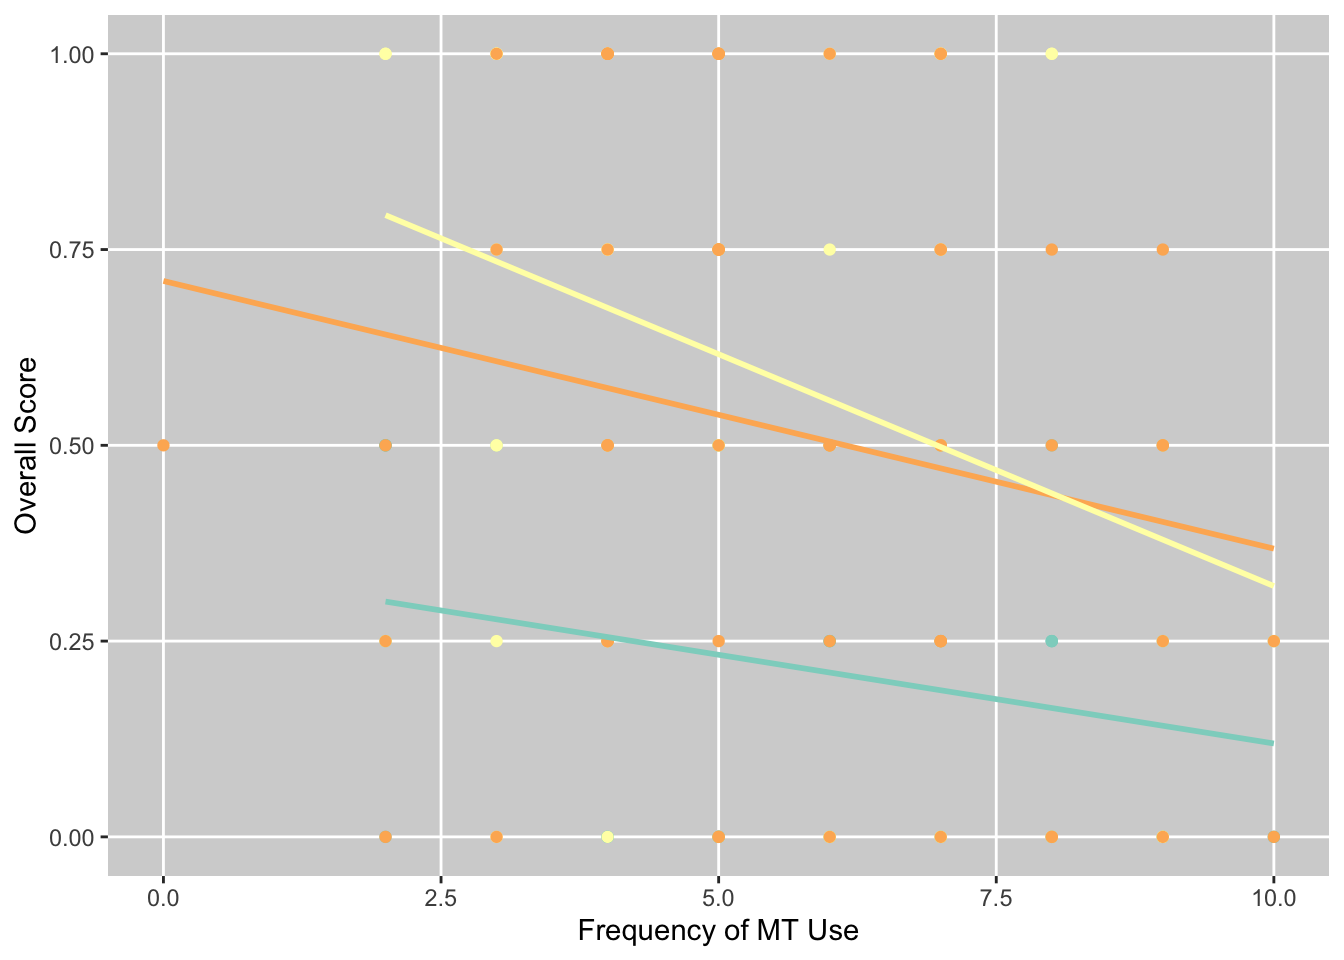
\includegraphics[width=0.95\textwidth]{images/exp2_MT_useage.png}
    \caption{Regression lines of overall score and frequency of MT usage by condition.}
    \label{fig:exp_MT_use}
    %\end{figure}
    
  \end{minipage}
\end{figure}

\paragraph{\textbf{Does intolerance of ambiguity affect performance?}} 

Given the survey instrument we use to measure Intolerance for Ambiguity\cite{gellerTolerance1993} participants’ scores could range from 7 (extremely low intolerance for ambiguity) to 49 (extremely high intolerance for ambiguity). In our study, the median score for participants' intolerance for ambiguity is 30. 

To determine if there could be a linear relationship between participants' $overall_score$ and $intolerance\_for\_ambiguity$, we test for a significant Pearson correlation between the two within each condition. Regression lines for each condition are shown in Figure \ref{fig:exp_intol_ambiguity}. We find no significant correlation in any condition (Human Quality -- ($r(57) = -0.14, p = 0.29$), Predicted Quality -- ($r(57) = 0.03, p = 0.81$), baseline -- ($r(45) = -0.01, p = 0.95)$), and thus do not perform any linear regressions. This suggests that intolerance for ambiguity does not have a significant effect on participants' performance, thus we \textbf{reject H3}. 

\paragraph{\textbf{Does regular usage of machine translation affect performance?}}

We ask participants to rank how often they use Google Translate and Facebook Translate on a five-point scale of Never, Yearly, Monthly, Weekly, Daily. We assign weights to each point on the scale ranging from 1 (Never) to 5 (Daily) and use these to calculate a machine translation usage score for each participant. The higher this score, the more often a participant indicates using MT. 

To determine if there could be a linear relationship between participants' $overall_score$ and $MT_usage$, we test for a significant Pearson correlation between the two within each condition.
Regression lines for each condition are shown in Figure \ref{fig:exp_MT_use}. We find a significant correlation between frequency of MT usage and overall score for participants in the Human Quality condition ($r(57) = -0.32, p < 0.05$), and no significant correlation in any other condition (Predicted Quality -- ($r(57) = -0.21, p = 0.11$), baseline -- ($r(45) = -0.23, p = 0.11$)). We run a linear regression for the Human quality condition and find a significant effect between $overall_score$ and $MT_usage$ ($F(1, 57) = 6.4, p < .05, R^2 = 0.10$), with $MT_usage$ as a significant predictor ($t = -2.54, p < 0.05$). This suggests that in the Human Quality condition, as participants’ frequency of MT usage increases, their performance decreases, thus we \textbf{partially accept H4}.

\begin{figure}[h!]
    \centering
    
    \cbox{bar-noXai} \textit{Baseline} \quad
    \cbox{bar-Qual} \textit{Human Quality} \quad
    \cbox{bar-PredictQ} \textit{Predicted Quality} \quad
    
    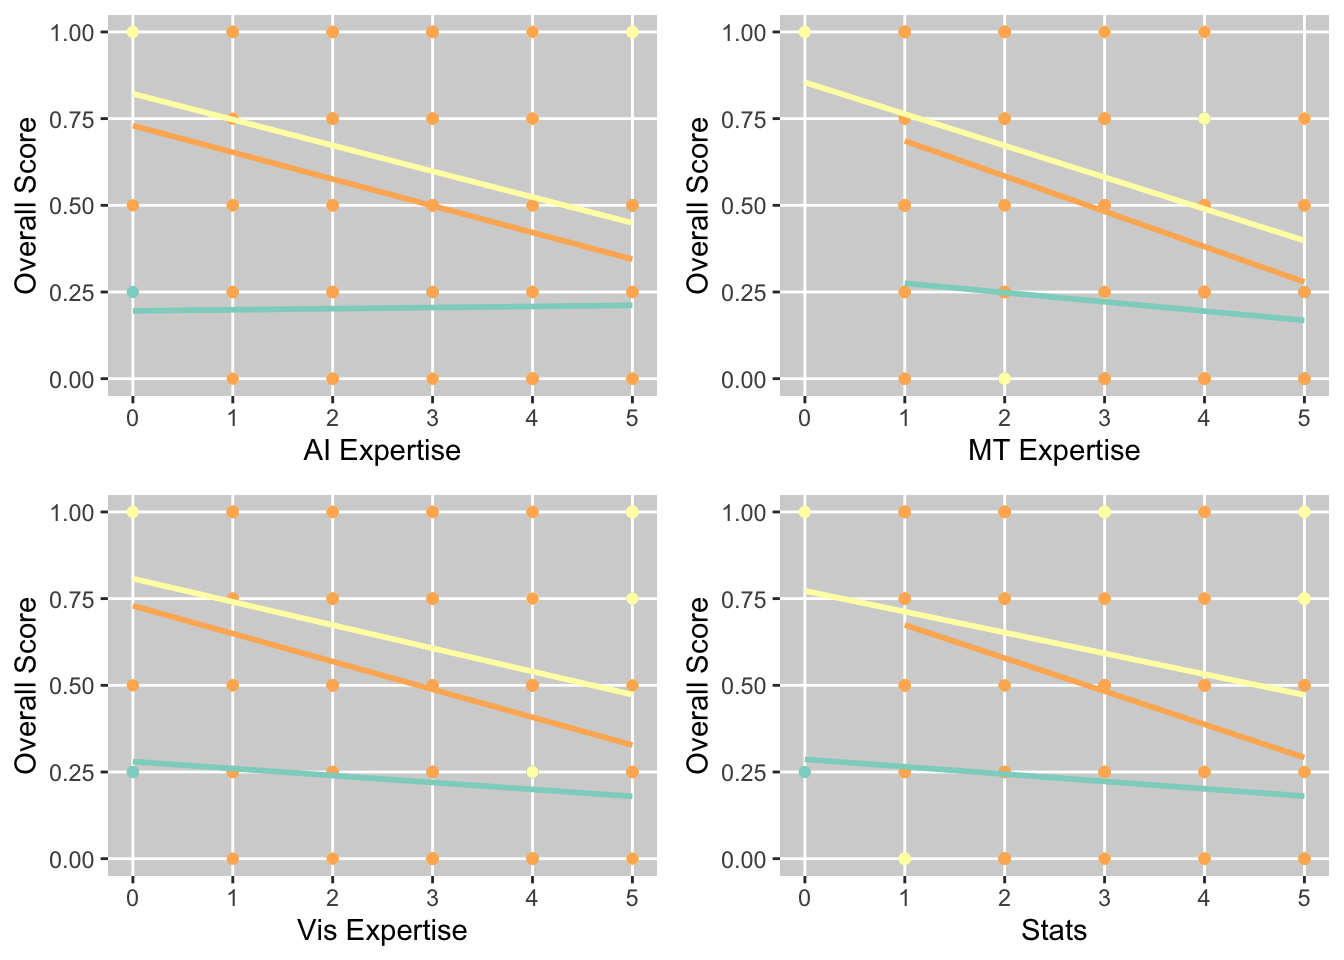
\includegraphics[width=0.50\textwidth]{exp2_expert.png}
    \caption{Regression lines of overall score and self-rated expertise by condition.}
    \label{fig:exp_expert}
\end{figure}

\begin{table}[h!]
\resizebox{0.90\textwidth}{!}{%
\begin{tabular}{llcc}
\hline
\multicolumn{1}{c}{Measure}                            & \multicolumn{1}{c}{Condition} & Result & Regression    \\ \hline
\multirow{4}{*}{Self-rated expertise in AI}            & Human Quality              & $\mathbf{r(57) = -0.27, p < 0.05}$ & 
$\mathbf{F(1, 57) = 4.39, p < 0.05, R^2 = 0.07; t = -2.10, p < 0.05}$  \\
                                                       & Predicted Quality          & $\mathbf{r(57) = -0.29, p < 0.05}$ & 
$\mathbf{F(1, 57) = 5.24, p < 0.05, R^2 = 0.08; t = -2.29, p < 0.05}$         \\
                                                       & Baseline                     & $r(45) = 0.02, p = 0.91$                     \\ \hline
\multirow{4}{*}{Self-rated expertise in MT}            & Human Quality              & $\mathbf{r(57) = -0.31, p < 0.05}$ & 
$\mathbf{F(1, 57) = 6.26, p < 0.05, R^2 = 0.10; t = -2.50, p < 0.05}$ \\
                                                       & Predicted Quality          & $\mathbf{r(57) = -0.40, p < 0.01}$ & 
$\mathbf{F(1, 57) = 10.55, p < 0.01, R^2 = 0.16; t = -3.25, p < 0.01}$          \\
                                                       & Baseline                     & $r(45) = -0.13, p = 0.39$                    \\ \hline
\multirow{4}{*}{Self-rated expertise in visualization} & Human Quality              & $r(57) = -0.24, p = 0.06$                    \\
                                                       & Predicted Quality          & $\mathbf{r(57) = -0.31, p < 0.05}$ & 
$\mathbf{F(1, 57) = 6.18, p < 0.05, R^2 = 0.10; t = -2.49, p < 0.05}$                  \\
                                                       & Baseline                     & $r(45) = -0.11, p = 0.48$                    \\ \hline
\multirow{4}{*}{Self-rated expertise in statistics}    & Human Quality              & $r(57) = -0.21, p = 0.10$                    \\
                                                       & Predicted Quality          & $\mathbf{r(57) = -0.36, p < 0.01}$ & 
$\mathbf{F(1, 57) = 8.75, p < 0.01, R^2 = 0.13; t = -2.96, p < 0.01}$          \\
                                                       & Baseline                     & $r(45) = -0.11, p = 0.46$                    \\ \hline
\end{tabular}%
}
\caption{Pearson correlation results for each self-rated expertise measure by condition. Significant results are in \textbf{bold} and regression results are included.}
\label{tab:exp1_expertise_stats}
\end{table}


\paragraph{\textbf{Does participants' self-rated expertise affect performance?}}

We ask participants to rate their own expertise from 1 (Novice) to 5 (Expert) in four areas: AI, MT, visualization, and statistics. 

To determine if there could be a linear relationship between participants' $overall_score$ and $expertise$, we test for a significant Pearson correlation between the two within each condition. Regression lines for each condition are shown in Figure \ref{fig:exp_expert}.
In the Human Quality, and Predicted Quality conditions we find significant correlations between self rated expertise in AI and MT and $overall\_score$. In addition, we find significant correlations between self-rated expertise in visualization and statistics and overall score in the Predicted Quality condition. In all of these cases, linear regression shows self-rated expertise is a significant predictor of $overall\_score$. 
(Analysis results for all of these tests are listed in Table \ref{tab:exp1_expertise_stats}.) Overall, our results suggest that in both quality score conditions, as self-rated expertise in AI and MT (and in the case of Predicted Quality, visualization and statistics) increase, $overall\_score$ decreases, thus we \textbf{accept H5}.


\subsection{\textbf{Qualitative Feedback}}

Qualitative feedback from our study indicates that users are satisfied with VeriCAT. We ask participants in the Predicted Quality condition if they would have liked to see any additional information and only 5 of the 59 ($8.5\%$) participants answered yes. We interpret this to indicate that VeriCAT provides adequate information for users to perform the experimental task.       

\subsection{Discussion} 

In running this experiment, we sought to test if VeriCAT's method of showing sentence-level quality scores improves users' performance in a task that asks them to identify poor quality machine translations. We find that both Human and Predicted quality scores significantly improve user performance compared to the baseline condition. In addition, we find that although user performance is slightly lower with Predicted Quality scores (generated by VeriCAT's QE model) compared to Human Quality scores (generated by DA of translations by humans), this difference is not significant. 

We do not find evidence that VeriCAT impacts how participants' respond to our questions regarding trust of MT. There are a few potential explanations for this. It may be that participants come into the experiment with prior skepticism of MT quality. Even when translation quality scores help them perform the experimental task more accurately, the scores may not necessarily change their perception of the trustworthiness of MT in general. It may also be that our experimental task is not realistic enough to force users to consider their trust of MT output. Future work should explore situations where the stakes for users are higher. For example, future studies might ask users to flag sentences as inappropriate based on MT, or whether they would re-post a passage based on the MT. Scenarios such as these may elicit a stronger evaluation of trust from participants.

Unlike participants in the Human Quality condition, we do not find a significant correlation between participants' overall score and frequency of MT use in the Predicted Quality condition. However, we do find a significant negative correlation between participants' self-rated expertise in AI and MT and overall score in the Human and Predicted Quality conditions.  

This finding is surprising, as we would expect people who are more familiar with MT through frequent usage to have a better understanding of its limitations. Similarly, we would expect people with more expertise in MT and AI to have a better understanding of MT limitations and of how to read and process quality indicators. We postulate that in both of these cases we are observing participants' overconfidence leading to errors. It may be that participants who use MT more often become more comfortable with it and, as a result, see less need to rely on quality scores to identify poor translations. It may also be that these participants are less invested in attempting to perform the task as directed. We postulate that the same is true of self-rated experts in MT and AI. I.e. that participants who think they are better at understanding the underlying mechanisms of MT may be more likely to rely on their own quality assessments instead of those shown by VeriCAT.

Our findings suggest that novices are more likely to follow quality score guidance, while those with more familiarity or expertise in the area may ignore the guidance of quality scores in favor of their own judgement. When designing interfaces, designers should pay specific attention to the differences between these populations and appreciate that their system design may need to accommodate different users in different ways. 

Overall, our findings indicate that VeriCAT provides contextual information about the quality of MT text that is useful and intuitive for users. In particular, we see that VeriCAT's quality scores can help users overcome situations in which fluency of translated text is a poor proxy for quality. Our hope is that future work will continue in this area to investigate additional methods to provide MT users helpful indications of reliability and trustworthiness.     



